\documentclass{jsreport}
\usepackage{graphicx, url, algorithm, algorithmic, float, booktabs, listings, color, pdfpages, amsmath, amssymb, latexsym, mathtools, ascmac, amsfonts, amsthm}
\lstset{
  basicstyle={\ttfamily},
  identifierstyle={\small},
  commentstyle={\smallitshape},
  keywordstyle={\small\bfseries},
  ndkeywordstyle={\small},
  stringstyle={\small\ttfamily},
  frame={tb},
  breaklines=true,
  columns=[l]{fullflexible},
  numbers=left,
  xrightmargin=0zw,
  xleftmargin=3zw,
  numberstyle={\scriptsize},
  stepnumber=1,
  numbersep=1zw,
  lineskip=-0.5ex
}
\usepackage[table,xcdraw]{xcolor}
\newtheorem{theo}{定理}[chapter]
\newtheorem{defi}{定義}[chapter]
\newtheorem{lemm}{補題}[chapter]
\newtheorem{prop}{命題}[chapter]
\newtheorem{coro}{系}[chapter]
\newcommand{\red}[1]{\textcolor{red}{#1}}
\newcommand{\blue}[1]{\textcolor{blue}{#1}}
\newcommand{\green}[1]{\textcolor{green}{#1}}
\renewcommand{\baselinestretch}{1.1}
\usepackage{mathrsfs}
\usepackage{bm}
\def\qed{\hfill $\Box$}
\usepackage{tikz}
\usetikzlibrary{intersections, calc, arrows}
\renewcommand\proofname{\bf 証明}

\begin{document}
\chapter{確率変数と確率分布}
\section{母集団と標本}
既知の無作為標本によって母集団の未知の性質を知ろうとすることを統計的推測 (statistical inference) という (図\ref{fig:inf}).
\begin{figure}[htb]
  \centering
  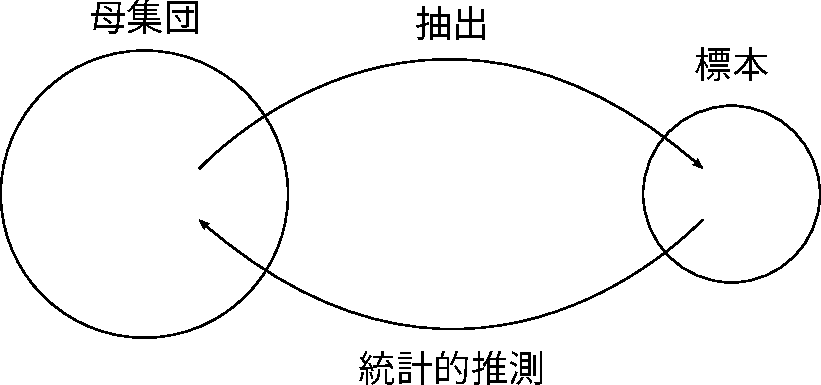
\includegraphics[clip, width=8cm]{../figure/infer.pdf}
  \caption{統計的推測のイメージ}
  \label{fig:inf}
\end{figure}

\section{確率変数と確率分布}
まず,離散型の確率変数とその分布を例に考える.$X$を2個のサイコロを投げたときに出た目の和を表す変数とする (表\ref{tab:ex_pr}).
\begin{table}[htb]
  \centering
  \caption{確率変数の例}
  \begin{tabular}{c|ccccc|c}
    $X$の値 & $2$ & $3$ & $4$ & $\cdots$ & $12$ & 計 \\ \hline
    確率 & $1/36$ & $2/36$ & $3/36$ & $\cdots$ & $1/36$ & $1$ \\ \hline
  \end{tabular}
  \label{tab:ex_pr}
\end{table}

この$X$のように,取りうる値に対して,確率が対応する変数を確率変数 (random variable) と呼ぶ.確率変数の取りうる値 (実現値) とその確率をペアにしたものを確率分布 (probability distribution) と呼ぶ.

一般に,確率変数$X$の実現値を$x_1, x_2, \ldots, x_n, \ldots$,その確率を$p_1, p_2, \ldots, p_n, \ldots$とすると,確率変数$X$の確率分布は,
\begin{equation}
  P(X = x_k) = p_k \; \; (k = 1, 2, \ldots)
\end{equation}
である.ただし,$\sum_{k = 1}^{\infty} p_k = 1, \, p_k \geq 0 \; (k = 1, 2, \ldots)$である.



\end{document}
